% Options for packages loaded elsewhere
\PassOptionsToPackage{unicode}{hyperref}
\PassOptionsToPackage{hyphens}{url}
%
\documentclass[
]{article}
\title{Exploratory Data Analysis}
\author{Ethan Allavarpu \(\cdot\) Raymond Bai \(\cdot\) Jaclyn Chiu
\(\cdot\) Ariel Chow \(\cdot\) Carlie Lin \(\cdot\) Dara
Tan \and \textbf{Explore the GLOBE}}
\date{Fall 2021}

\usepackage{amsmath,amssymb}
\usepackage{lmodern}
\usepackage{iftex}
\ifPDFTeX
  \usepackage[T1]{fontenc}
  \usepackage[utf8]{inputenc}
  \usepackage{textcomp} % provide euro and other symbols
\else % if luatex or xetex
  \usepackage{unicode-math}
  \defaultfontfeatures{Scale=MatchLowercase}
  \defaultfontfeatures[\rmfamily]{Ligatures=TeX,Scale=1}
\fi
% Use upquote if available, for straight quotes in verbatim environments
\IfFileExists{upquote.sty}{\usepackage{upquote}}{}
\IfFileExists{microtype.sty}{% use microtype if available
  \usepackage[]{microtype}
  \UseMicrotypeSet[protrusion]{basicmath} % disable protrusion for tt fonts
}{}
\makeatletter
\@ifundefined{KOMAClassName}{% if non-KOMA class
  \IfFileExists{parskip.sty}{%
    \usepackage{parskip}
  }{% else
    \setlength{\parindent}{0pt}
    \setlength{\parskip}{6pt plus 2pt minus 1pt}}
}{% if KOMA class
  \KOMAoptions{parskip=half}}
\makeatother
\usepackage{xcolor}
\IfFileExists{xurl.sty}{\usepackage{xurl}}{} % add URL line breaks if available
\IfFileExists{bookmark.sty}{\usepackage{bookmark}}{\usepackage{hyperref}}
\hypersetup{
  pdftitle={Exploratory Data Analysis},
  pdfauthor={Ethan Allavarpu \textbackslash cdot Raymond Bai \textbackslash cdot Jaclyn Chiu \textbackslash cdot Ariel Chow \textbackslash cdot Carlie Lin \textbackslash cdot Dara Tan; },
  hidelinks,
  pdfcreator={LaTeX via pandoc}}
\urlstyle{same} % disable monospaced font for URLs
\usepackage[margin=1in]{geometry}
\usepackage{graphicx}
\makeatletter
\def\maxwidth{\ifdim\Gin@nat@width>\linewidth\linewidth\else\Gin@nat@width\fi}
\def\maxheight{\ifdim\Gin@nat@height>\textheight\textheight\else\Gin@nat@height\fi}
\makeatother
% Scale images if necessary, so that they will not overflow the page
% margins by default, and it is still possible to overwrite the defaults
% using explicit options in \includegraphics[width, height, ...]{}
\setkeys{Gin}{width=\maxwidth,height=\maxheight,keepaspectratio}
% Set default figure placement to htbp
\makeatletter
\def\fps@figure{htbp}
\makeatother
\setlength{\emergencystretch}{3em} % prevent overfull lines
\providecommand{\tightlist}{%
  \setlength{\itemsep}{0pt}\setlength{\parskip}{0pt}}
\setcounter{secnumdepth}{-\maxdimen} % remove section numbering
\ifLuaTeX
  \usepackage{selnolig}  % disable illegal ligatures
\fi

\begin{document}
\maketitle

\hypertarget{the-data}{%
\section{The Data}\label{the-data}}

The data set we have chosen to analyze is the \textbf{Dana Landis
Leadership} dataset, which comes from the GLOBE Research Survey. The
data provided in the folder had survey results for (1) leadership and
(2) societal and culture data and a PDF describing the nature of the
survey, but nothing else. To glean more information, we found the two
questionnaires (alpha and beta) described in the informational PDF to
get the original questions. While we do not have a ``codebook'' in the
traditional sense, the original questions asked may help guide us in
understanding what each variable means and how the survey represents
respondents' answers numerically. The survey is on a 1 to 7 scale, with
1 being a negative response, 4 a ``neutral'' score, and 7 positive.

\hypertarget{leadership}{%
\section{Leadership}\label{leadership}}

\begin{center}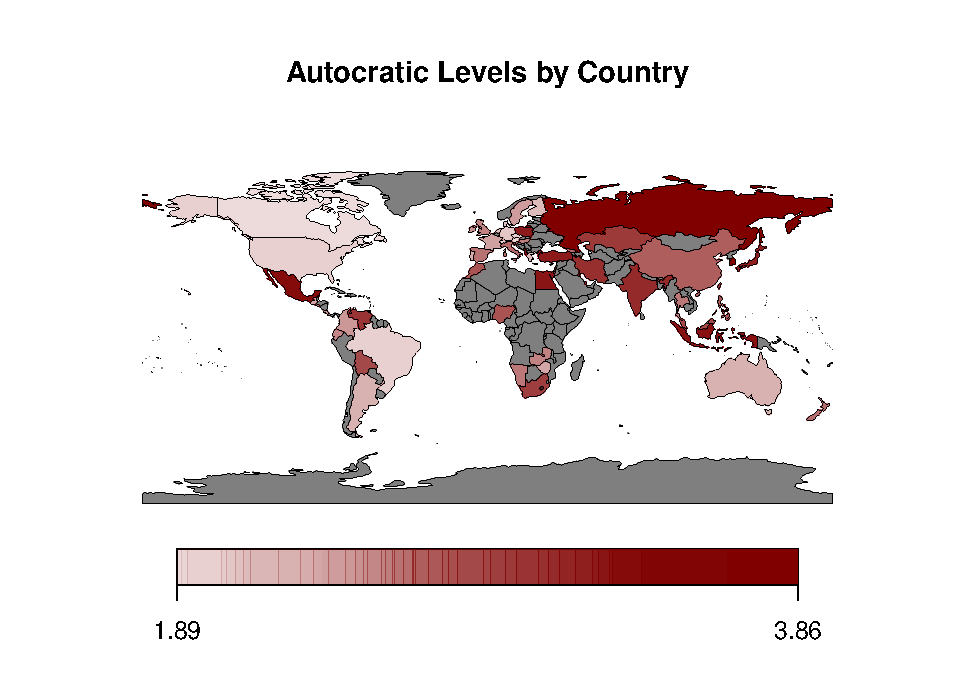
\includegraphics[width=0.95\linewidth]{eda_files/figure-latex/leadership-1} \end{center}

The above global heatmap presents the beliefs about whether autocracy
helps (higher values) or hinders (lower values) leaders in a given
country. Multiple similar graphics were generated for a variety of
leadership variables, ultimately leading us to recognize that different
regions of the world may favor certain leadership qualities over others
and that certain leadership qualities may be liked/disliked ``together''
(i.e., they have associations).

From boxplots we generated (not pictured), the difference by country
cluster (as defined by the dataset) seems visible, prompting us to
consider clustering countries to determine how they may be separated. We
do want to note that there are only 62 observations--this totals to
fewer than 62 countries because Germany and South Africa have two
observations each (West vs.~East and White vs.~Black, respecively). The
limited number of observations may limit us in the scope of our analysis
because we have less than a third of the total countries (demonstrated
by the vast swaths of grey on the world map for which there is no data)
and clustering would further reduce block/group sizes.

\hypertarget{societal-values-and-practices}{%
\section{Societal Values and
Practices}\label{societal-values-and-practices}}

\begin{center}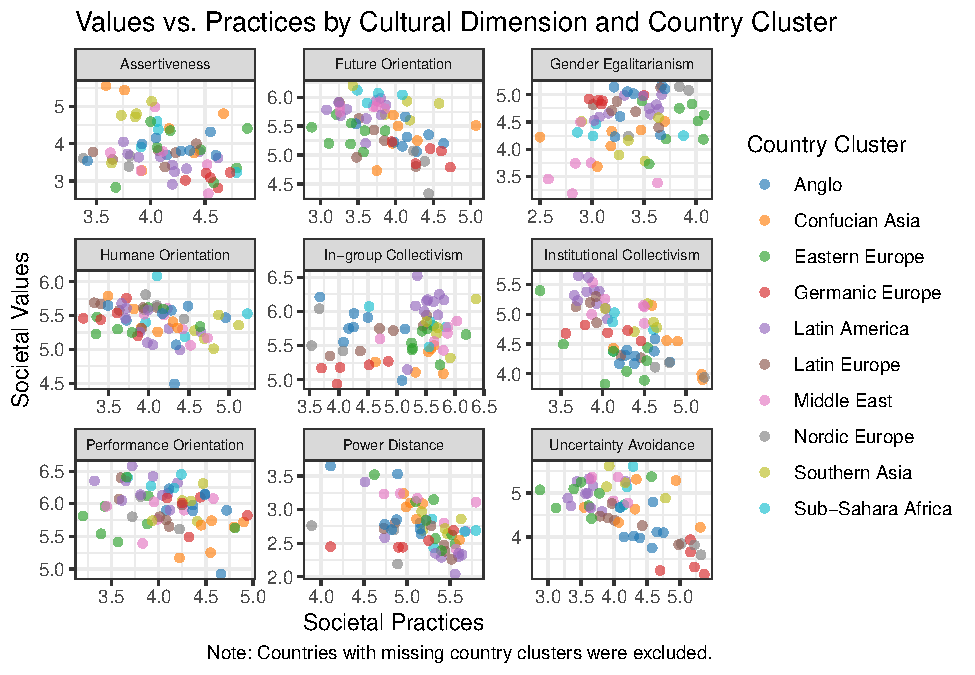
\includegraphics{eda_files/figure-latex/society-1} \end{center}

The plot grid demonstrates how, contrary to what \emph{should} happen,
the societal values of a country do not correlate well with the societal
practices (what \emph{should be} does not align with what \emph{is}).
This may be a source of further exploration, as we may want to see
whether there is a significant difference between the values and
practices. When we look at the per-region divisions though (by color),
the trend (or lack thereof) seems to persist for these concepts.

\hypertarget{problem-statements}{%
\section{Problem Statements}\label{problem-statements}}

From the above exploratory analysis, we see that the data have been
segregated into two sets: those regarding leadership beliefs (i.e., what
makes a good leader) and those about society (values, practices, and
beliefs). Thus, to mirror this, we have two main problem statements we
want to consider:

\begin{enumerate}
    \item Which characteristics or traits do countries tend to group together when determining ``good" leadership values?
    \item Do societal practices and societal values align?
    \begin{itemize}
        \item If they do not, which practices and values deviate most significantly?
    \end{itemize}
\end{enumerate}

\hypertarget{potential-issues}{%
\section{Potential Issues}\label{potential-issues}}

While promising, there are a few issues with the data that we have to
consider. First, the number of observations: 62 observations is a rather
small dataset, which suggests that any analysis will likely be limited.
Another potential issue is running multiple significance tests: with
nine societal practice vs.~value concepts to consider, maintaining the
\(\alpha = 0.05\) significance level would increase the experimentwise
error rate and thus the likelihood of a false positive
(\(P(\text{False Positive}) = 1 - P(\text{No False Positive}) = 1 - 0.95^{9} \approx 0.3698\)).
To remedy this issue, we may either consider employing a
\emph{Bonferroni correction} or \emph{Tukey's method (HSD).}

\end{document}
